   
\documentclass[11pt]{article}
\usepackage{amsmath,amsthm,verbatim,amssymb,amsfonts,amscd, graphicx}
\usepackage{graphicx}
\usepackage{listings}
\usepackage{float}
\usepackage{url}
\usepackage{titlesec}
\setcounter{secnumdepth}{4}




\graphicspath{{./times/}}
\topmargin0.0cm
\headheight0.0cm
\headsep0.0cm
\oddsidemargin0.0cm
\textheight23.0cm
\textwidth16.5cm
\footskip1.0cm

\titleformat{\paragraph}
{\normalfont\normalsize\bfseries}{\theparagraph}{1em}{}
\titlespacing*{\paragraph}
{0pt}{3.25ex plus 1ex minus .2ex}{1.5ex plus .2ex}


\begin{document}
\title{CS 5220\\ Project 2 - Shallow Water Simulation}
\author{Marc Aurele Gilles (mtg79)\\ Sheroze Sheriffdeen(mss385)}
\maketitle

\section{Introduction}

The goal of this project to profile, parallelize and tune a particular structured grid computation: a shallow-water equations solver.  \\

The shallow-water equations are a two-dimensional PDE system that describes waves that are very long compared to the water depth. The variables of the PDE system are the water height $h$, and the velocity components $(u,v)$. The governing equations are \\

$$U_t = F(U)_x + G(U)_y)$$
where 
$$U = \begin{bmatrix}
h \\
hu \\
hv
\end{bmatrix}
,
F = \begin{bmatrix}
hu \\
h^2u+gh^2/2 \\
huv
\end{bmatrix}
,
G=
\begin{bmatrix}
hv \\
huv \\
h^2v+gh^2/2
\end{bmatrix}
$$


\section{Design Decisions}

The following sections describe the implementation changes from the original code found at \url{https://github.com/cornell-cs5220-f15/water}. The current stable solution can be found at \url{https://github.com/sheroze1123/water/tree/vector_parallel} branch. 

\subsection{Memory Layout}
The original solution a two dimensional vectors of 3-vectors to represent $U_t$, $F(U)_x$, and $G(U)_y$. During each time step, the solution accesses each element in the 2-D grid sequentially. Then, the \texttt{vector<vector<real>>} representation leads to memory accesses that are not local spatially. \\

Therefore, our solution chooses to use 3 separate two dimensional vectors per objects, $U_t$, $F(U)_x$, and $G(U)_y$. Thus, we are required in general to perform three loop iterations in place of a single loop in the original solution. But this approach leverages spatial locality, especially in \texttt{compute\_step} and \texttt{limited\_derivs} functions.

\subsection{Vectorization}

By observing the profiling information, we noticed that the original solution spends majority of its computational time in the functions \texttt{limited\_derivs}, \texttt{compute\_step} and \texttt{compute\_fg\_speeds}. By adopting the newer memory layout, we enabled spatially local memory accesses. We were also able to decompose \texttt{for} loops in the solution to improve vectorization. Refer to \texttt{ipo\_out\_vectorization.optrpt} in \url{https://github.com/sheroze1123/water/tree/vectorization} for more information. \\

In \texttt{compute\_fg\_speeds}, we performed two separate loops to compute flux and wave speeds. The flux computation and the wave speed computation for the complete grid is not handled by the \texttt{Physics} class. We used \texttt{\#pragma simd} directives to instruct the compiler the ability to vectorize these computations. The compiler was successfully able to vectorize these functions with an estimated potential speedup of 6.7. \\

\texttt{limited\_derivs} uses the \texttt{limdiff} function in \texttt{minmod.h}. To improve the vectorization of this computation, we changed the implementation of \texttt{limdiff} in the following ways. 

\begin{enumerate}
	\item \texttt{limdiff} now performs the computation on the complete grid instead of at one grid point.
	\item \texttt{limdiff} was decomposed as \texttt{limdiff\_x} and \texttt{limdiff\_y} to perform the limiter along the $x$ dimension and the $y$ dimension separately while still retaining unit stride. 
\end{enumerate}

\subsection{Parallelization}
The updated memory layout is amenable to parallelization via OpenMP, particular during the costly operations of \texttt{limited\_derivs} and \texttt{compute\_step}. \\

At the beginning of a call to \texttt{limited\_derivs} we initialize a team of threads using \texttt{\#pragma omp parallel}. Each application of the limiter to the components of $U_t$, $F(U)_x$, and $G(U)_y$ can be computed in parallel since we removed the data dependencies by creating 3 separate two dimensional arrays per component. We use the \texttt{\#pragma omp for} directive to parallelize the grid computation of each component. \\

In \texttt{compute\_step}, we initialize a team of threads using \texttt{\#pragma omp parallel}. The predictor step is now performed in parallel. Then, we create a barrier before proceeding to the corrector step since the the corrector step needs information from the predictor. After computing the corrector step, we perform a barrier before finally copying back to storage in parallel. The performance increase we observed via parallelization reached up to 3+ speedup. Results are plotted in section~\ref{sec:speedup}.


\subsection{Domain Decomposition}


\subsubsection{General Setup}
We decomposed the main grid into equally sized sub-grids, by first copying  each sub-grid into a separate array. Each sub-grid array contains its part of the main grid an outer layer of ghost cells which contain information about the neighboring cells or the cells on the opposite side of the main grid if the sub-domain is close to the boundary of the main grid as we use periodic boundary condition. We then perform some number of time steps on each independent sub-grid and finally synchronize by copying back the sub-grid (without the ghost cells) onto the main grid. 

\subsubsection{Ghost cells}

The width of the layer of ghost cells for each sub-grid is $1.5t$, where t is the number of time steps we wish to advance before synchronizing back onto the main grid. For each sub-grid, we declare a simulation object, and run the simulation essentially in the same manner as we would on the whole grid, except we never apply periodic boundary conditions on the sub-grids. Because of this, at each two time steps we perform without synchronization, we "loose" 3 layers of ghost cells, in the sense that the computation within this layer is erroneous. \\

However, the rest of the grid is not contaminated with error, as information spreads through our simulation only by 3 layers per 2 time steps.

\subsubsection{Estimating the wave speed}
The main barrier to in adopting domain decomposition parallelization for this simulation is that we need to estimate the wave speed at each time step to be able to estimate a how big of a time step we can perform for the next iteration. Hence to allow each sub-grid to run from time $t=0$ to time $t=t_{final}$, we would need know in advance the speeds at time $t$, $t + dt_1$, $t + (dt_1+dt_2)$ ... $t+\sum_{i=1}^{k-1}dt_i$. But we obviously do not have access to those speeds at time $t$. \\

The problem is that we need to know at least an upper bound on the wave speed at each time step to be able to decide how many time steps it will take to reach $t_{final}$, as the number of time steps needed is directly proportional to the number of ghost cells we need to allocate for each sub-grid at time $t$. Our solution is to estimate an upper bound on the max wave speed, set the max wave speed for the next $k$ iterations to a be a multiple $r$ of the speed of the wave at time $t$ which we can compute before parallelizing. (in our code, we set $r=1.5$). \\

Furthermore, for each sub grid at each time checks independently if the wave speed on the subdomain is greater than our bound, if it is the case our program throws an error and stops. This failure check occurs locally to each thread, so there is no need for synchronization. 

\subsubsection{Avoiding Race conditions}
In order to avoid the race condition that can occur by a thread mapping back the state of the simulation on a later time steps onto the main grid before another thread got to copy from the main grid the simulation at the current time step, we use two different main grid (main grid 1 and main grid 2). At the first iteration (which computes multiple time steps), all thread copy from main grid 1, do computations, and write onto main grid 2. When the first iteration is done, all thread copy from main grid 2, do computations, and write onto main grid 1. We alternate between the grids in this manner until we have reached tfinal, making sure that the final state is written onto main grid 1 (which is passed to the driver function). In this manner, we avoid race conditions between the threads, and keep the synchronization costs to a minimum.



\subsubsection{Choosing a number of time steps}
The size of the computation that each subgrid has to do for each time steps depends on the number of time steps it has to accomplish before synchronizing back to the main grid. Specifically, the subgrid with ghost cells have sizes
$(n+2(t\frac{3}{2}+3))^2$ where n is the size of the part of the main grid that is assigned to that the subgrid, and t is the number of time steps taken before synchronization. The 3/2 factor is due to the fact that the information spreads at the rate of 3 layers per 2 time steps in our computation, the 2 factor to account for the the fact that we need one layers on each side of the grid, and the constant 3 is implementation dependent. We use the following heuristic to choose the number of time steps that we perform: the work per time steps on the subgrid with ghost cells has to be at most a multiple $c$ (in our code, we use $c=1.5$) of the work that would be performed on the subgrid alone (with no ghost cells). This leads us to the inequation:
$$ (n+2(t\frac{3}{2}+3))^2 \leq c n^2$$
A few algebra steps lead us to:
$$ t \leq \frac{(\sqrt c-1)n}{3}-2$$
We choose the largest even number t that satisfies this bound, or 2, whichever is largest.
 

\section{Analysis}
\subsection{Profiling} \label{sec:prof}

The following time profiles were obtained on a 200x200 grid by advancing 100 frames. 

\subsubsection{Original solution}
We began the optimization by analyzing the time profiles of the original code. The following table shows the top 4 functions by CPU time. We note that the bottleneck in the original solution lies in \texttt{limited\_derivs} and \texttt{compute\_step}.
\lstinputlisting[basicstyle=\tiny]{./profiling/original.txt}

\subsubsection{Vectorization}
Profiling of vectorization shows good improvements in performance, especially in the \texttt{limited\_derivs} and \texttt{compute\_fg\_speeds} functions, but a reduction in performance in the \texttt{compute\_step} function. The repetition of \texttt{limdiff\_x} and \texttt{limdiff\_y} is due to separation of components and axes in \texttt{limited\_derivs}. 
\lstinputlisting[basicstyle=\tiny]{./profiling/vectorization.txt}

\subsubsection{Parallelization}
For parallelization, we list the functions that take up the most CPU time and their associated OpenMP spin times. Although we see speedups in the parallel code, the profiling shows that we spend a lot of CPU time spinning. This indicates load imbalance issues in our code that we aim to address in the final report. 

\lstinputlisting[basicstyle=\tiny]{./profiling/vector_parallel_small.txt}

\subsection{Scaling Study} \label{sec:speedup}


\subsubsection{Strong Scaling Study}
We observe the speedup with respect to the number of threads in our parallel implementation. Here, speedup $s$ is defined to be,  

\begin{equation}
	\mathrm{s} = \dfrac{t_{parallel}}{t_{serial}}
\end{equation}

\paragraph{Parallel approach with vectorization}

Following is the strong scaling study where we solve the problem using a single domain with parallelization and vectorization. We solve the problem on a 500x500 grid for 100 frames. The observed best performance occurs when the number of threads are $\approx10$. Increasing the number of threads further results in plateauing in speedup which can be attributed to extra threads not being employed due to limited parallelization. The plateau is lower than the observed maximum speedup. We believe that this is due to thread scheduling overhead. Note that the original solution has a speedup $< 1$ in the following plot. The implementation of this version can be found at the \texttt{vector\_parallel} branch.

\begin{figure}[H]
    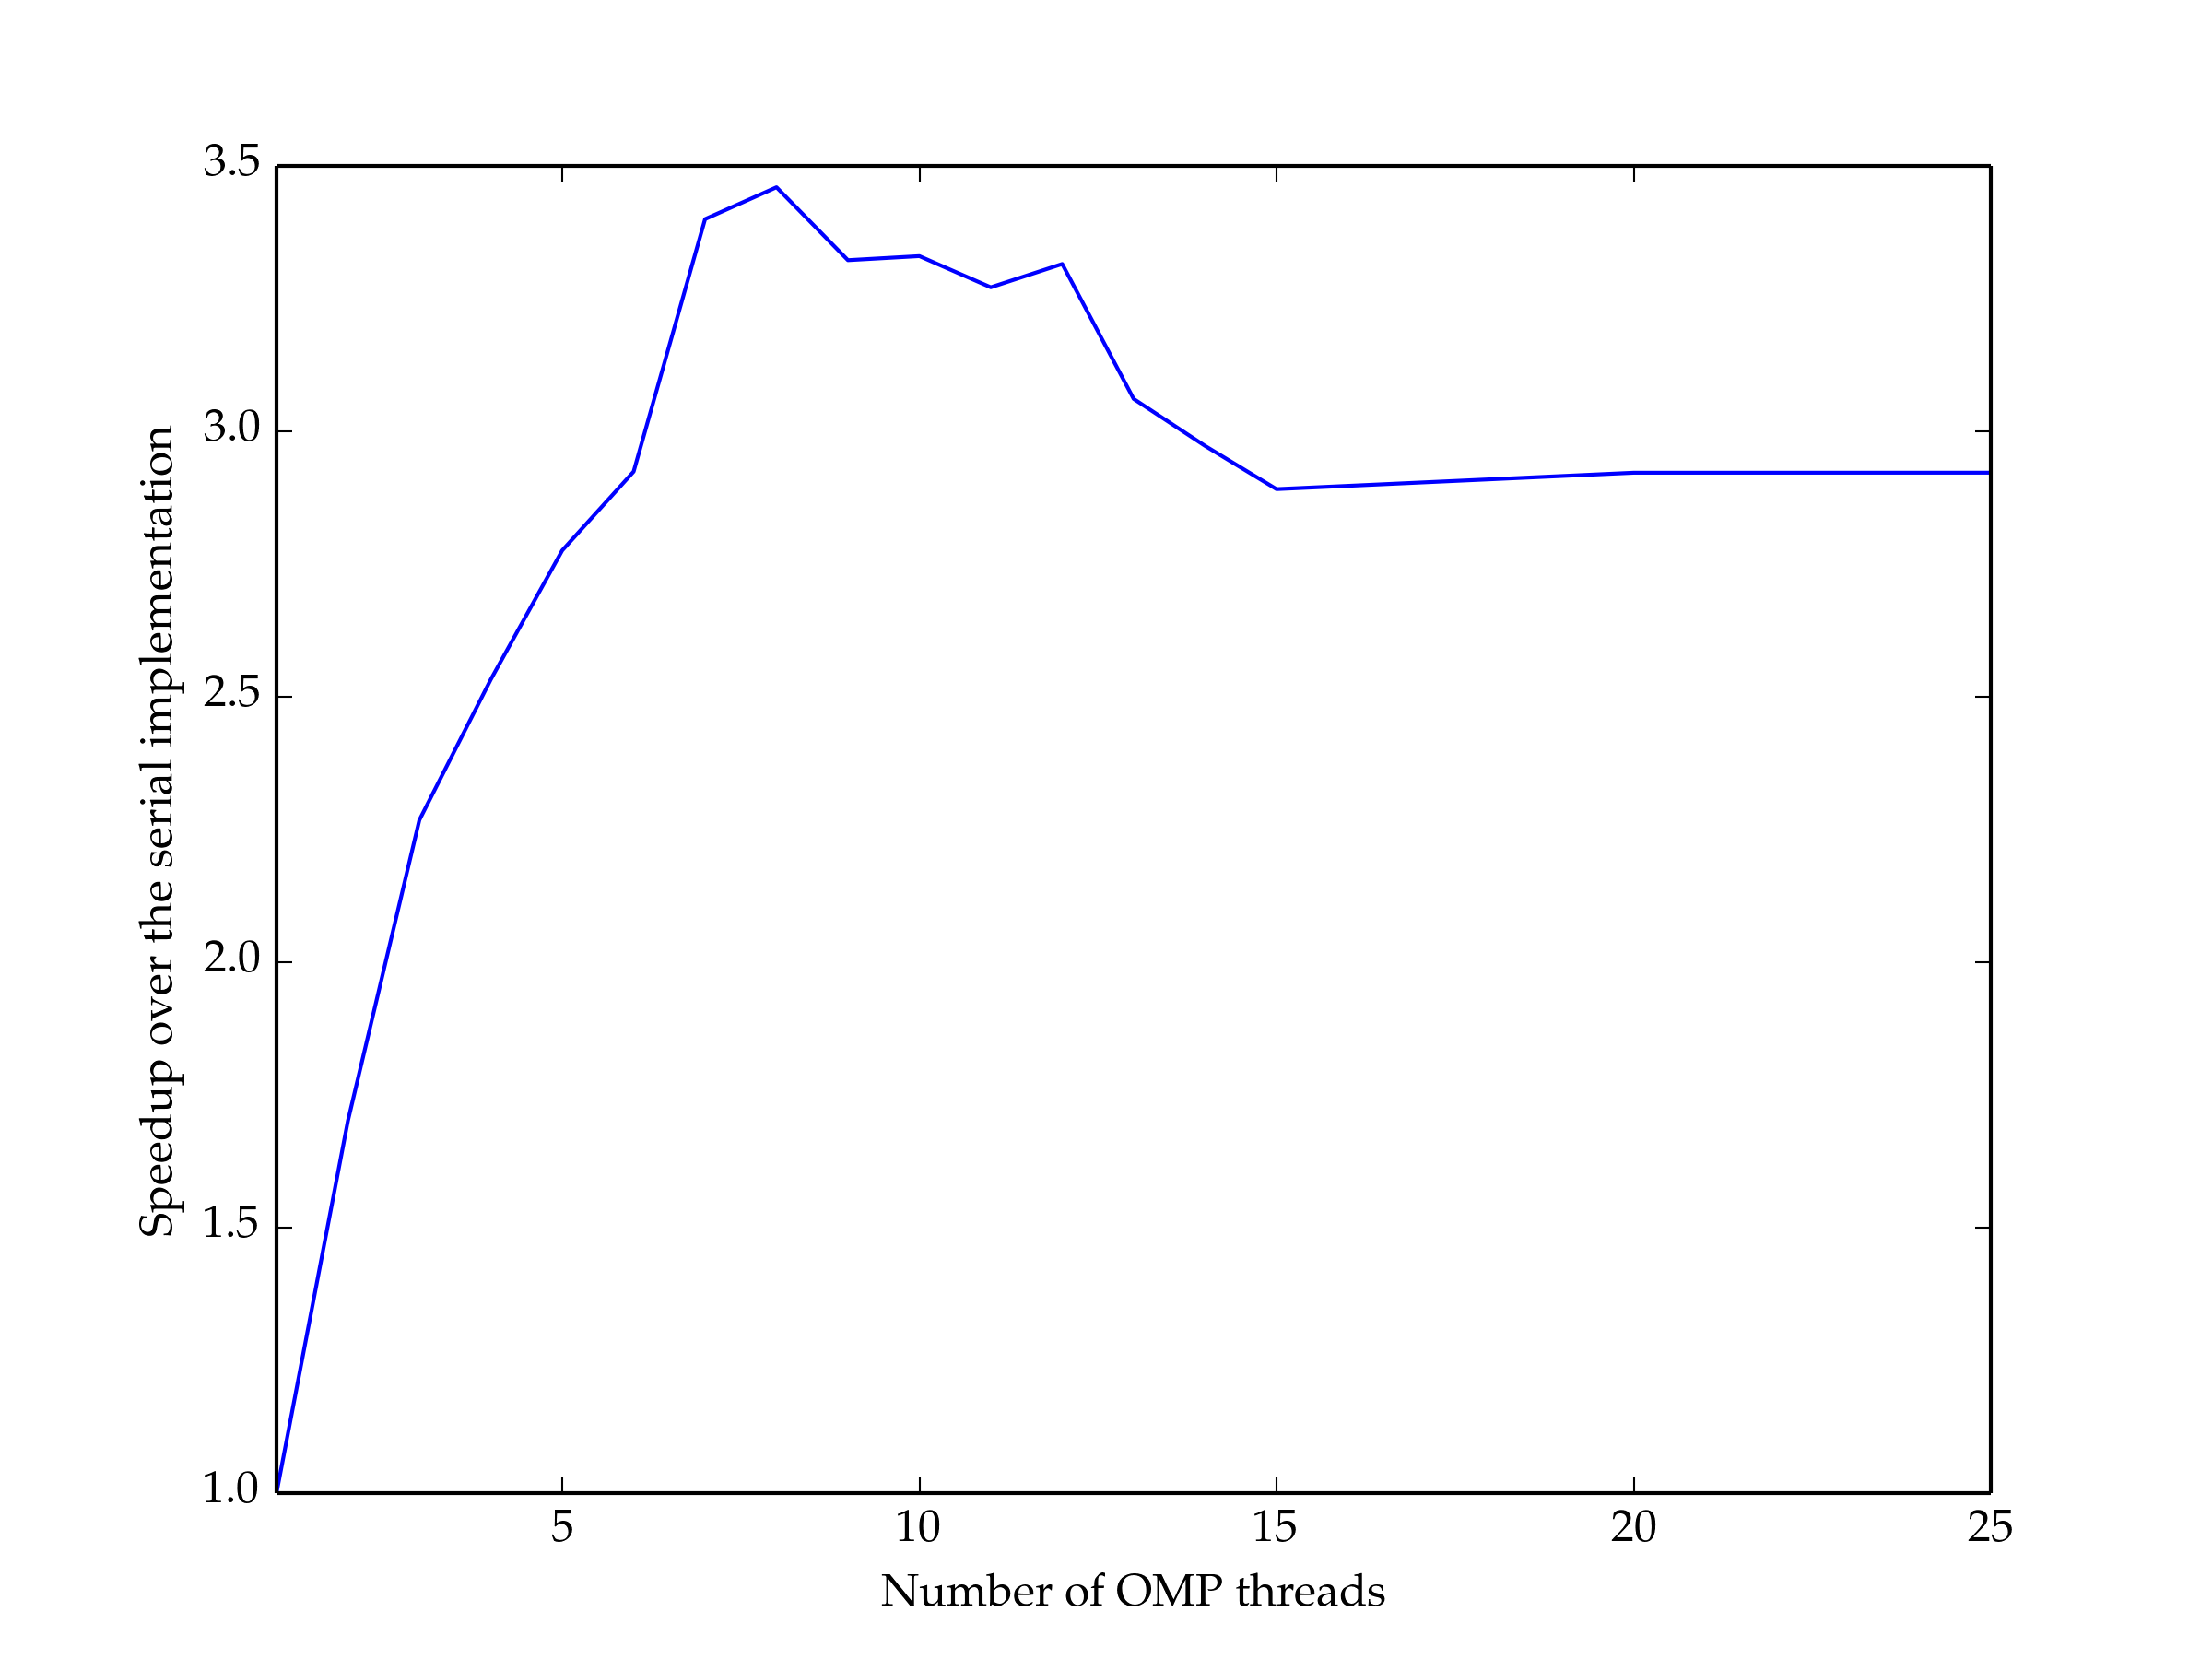
\includegraphics[width=0.9\textwidth]{./strong_scaling/strong_scaling_vector_parallel.png}
    \caption{Speedup as a function of the number of threads}
    \label{fig:strong_scaling}
\end{figure} 


\paragraph{Parallel domain decomposition}

The strong scaling study for the domain decomposed version of the solution shows good speedup with increasing number of threads. The problem was solved on a 1000x1000 grid for 100 frames. The implementation can be found at the \texttt{spatial\_vector\_merge} branch.

\begin{figure}[H]
    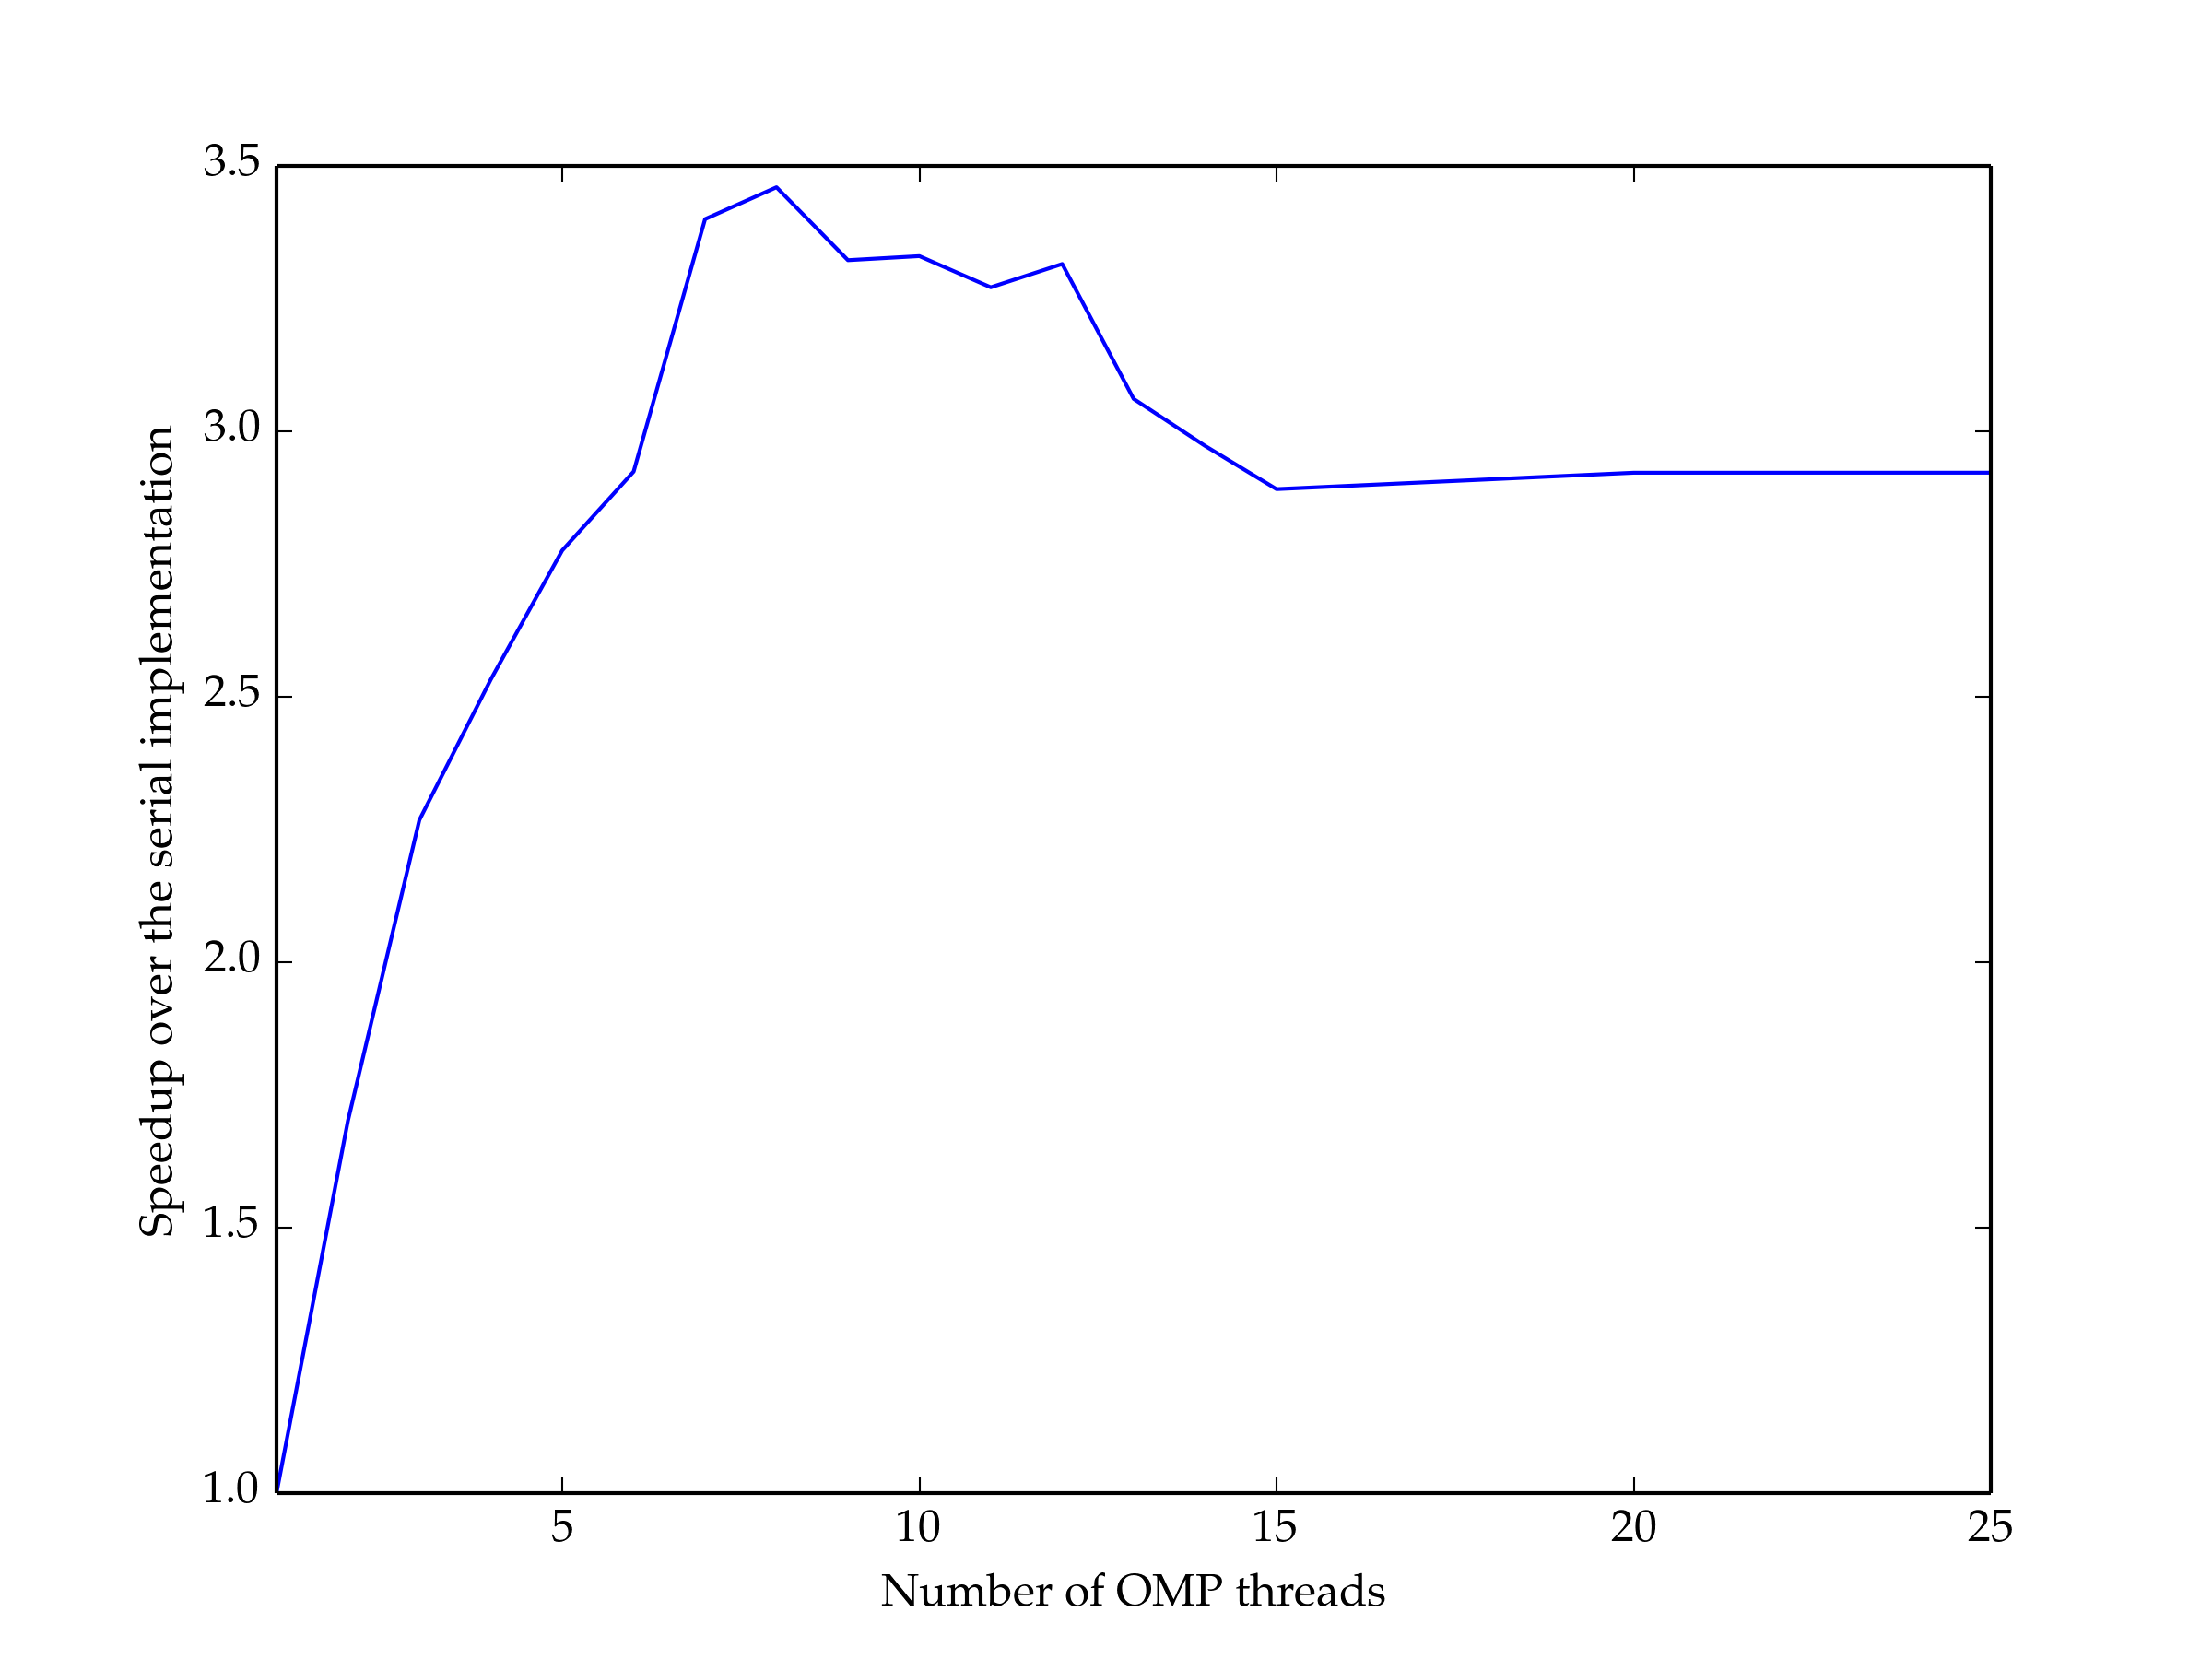
\includegraphics[width=0.9\textwidth]{./strong_scaling/strong_scaling.png}
    \caption{Speedup as a function of the number of threads}
    \label{fig:strong_scaling_dd}
\end{figure} 


\subsubsection{Weak Scaling Study}

We vary the threads but keep the problem size per thread constant. In figure~\ref{fig:weak_scaling}, each thread ideally computes a sub-problem equivalent to advancing a 300 x 300 grid by 100 frames. We 
plot the speedup observed while increasing the number of threads and the problem size such that work done per thread is approximately equal. 

\paragraph{Parallel approach with vectorization}

In the single domain, parallelized approach, we observe a exponential decrease in speedup per core. We believe that this can be attributed to load imbalance between threads and thread scheduling overhead. The implementation of this version can be found at the \texttt{vector\_parallel} branch.
 

 \begin{figure}[H]
    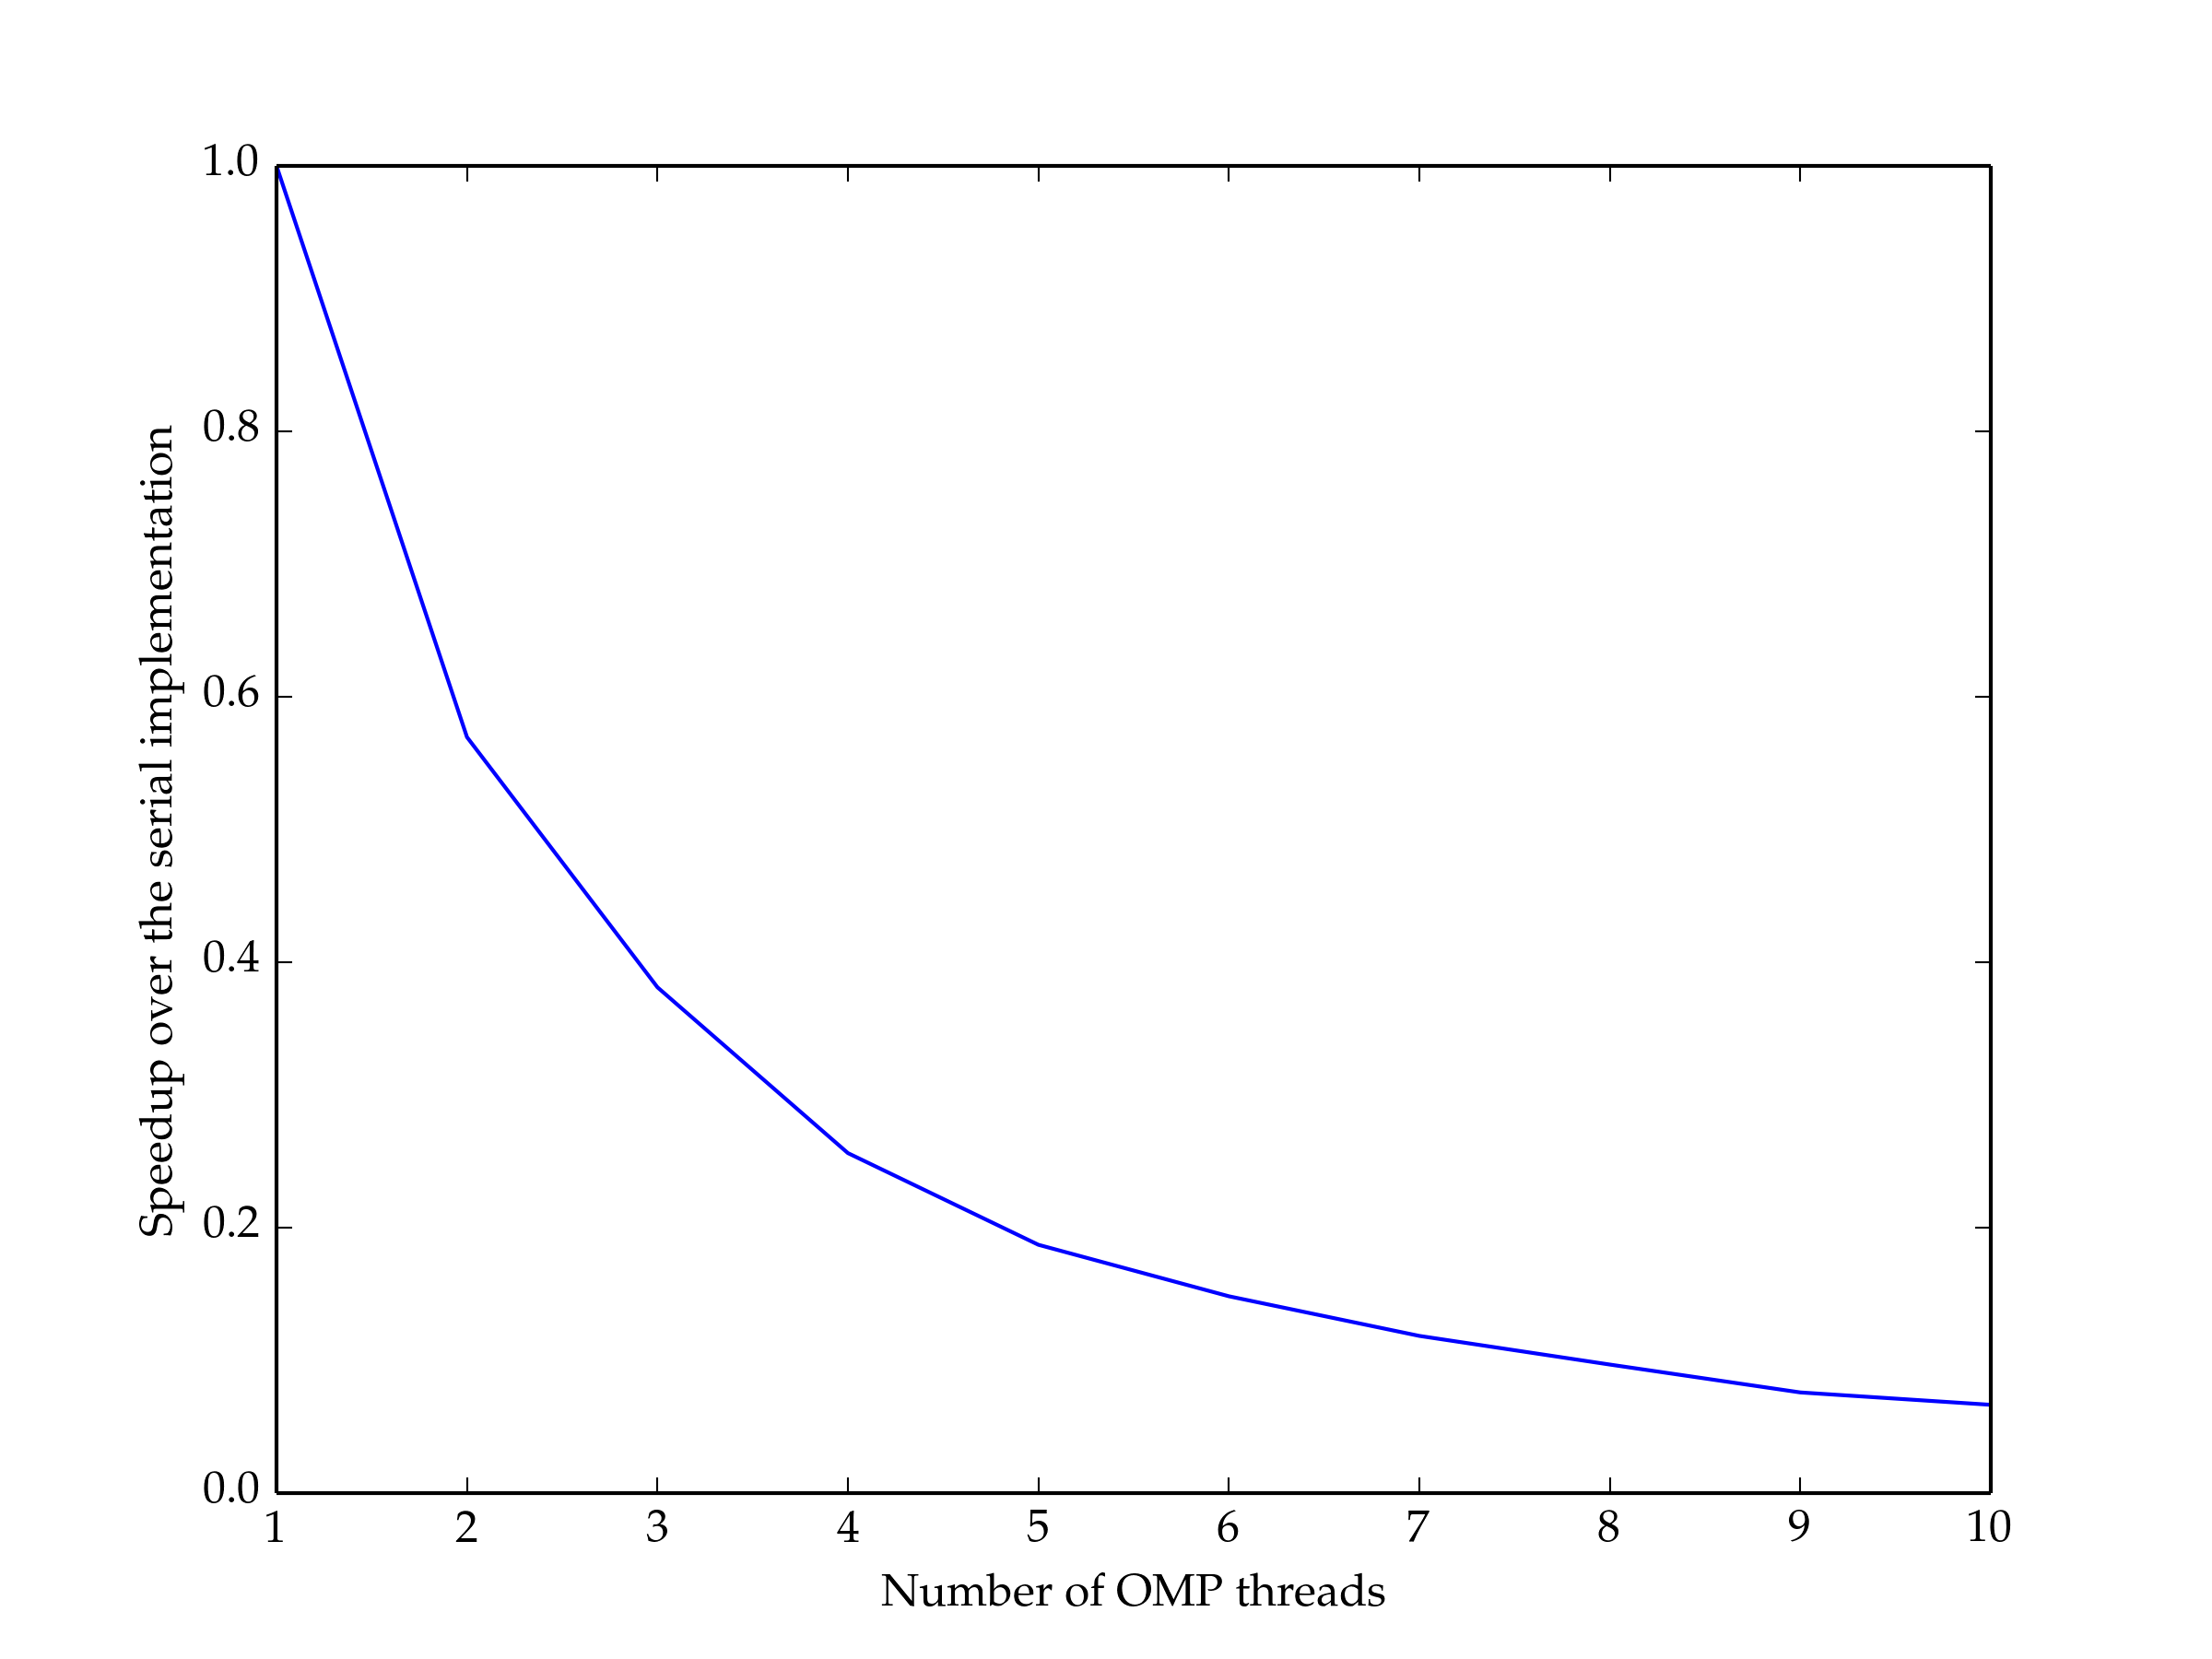
\includegraphics[width=0.9\textwidth]{./weak_scaling/weak_scaling_vector_parallel.png}
    \caption{Speedup as a function of the number of threads}
    \label{fig:weak_scaling}
\end{figure} 

\paragraph{Parallel domain decomposition}

The implementation can be found at the \texttt{spatial\_vector\_merge} branch.

 \begin{figure}[H]
    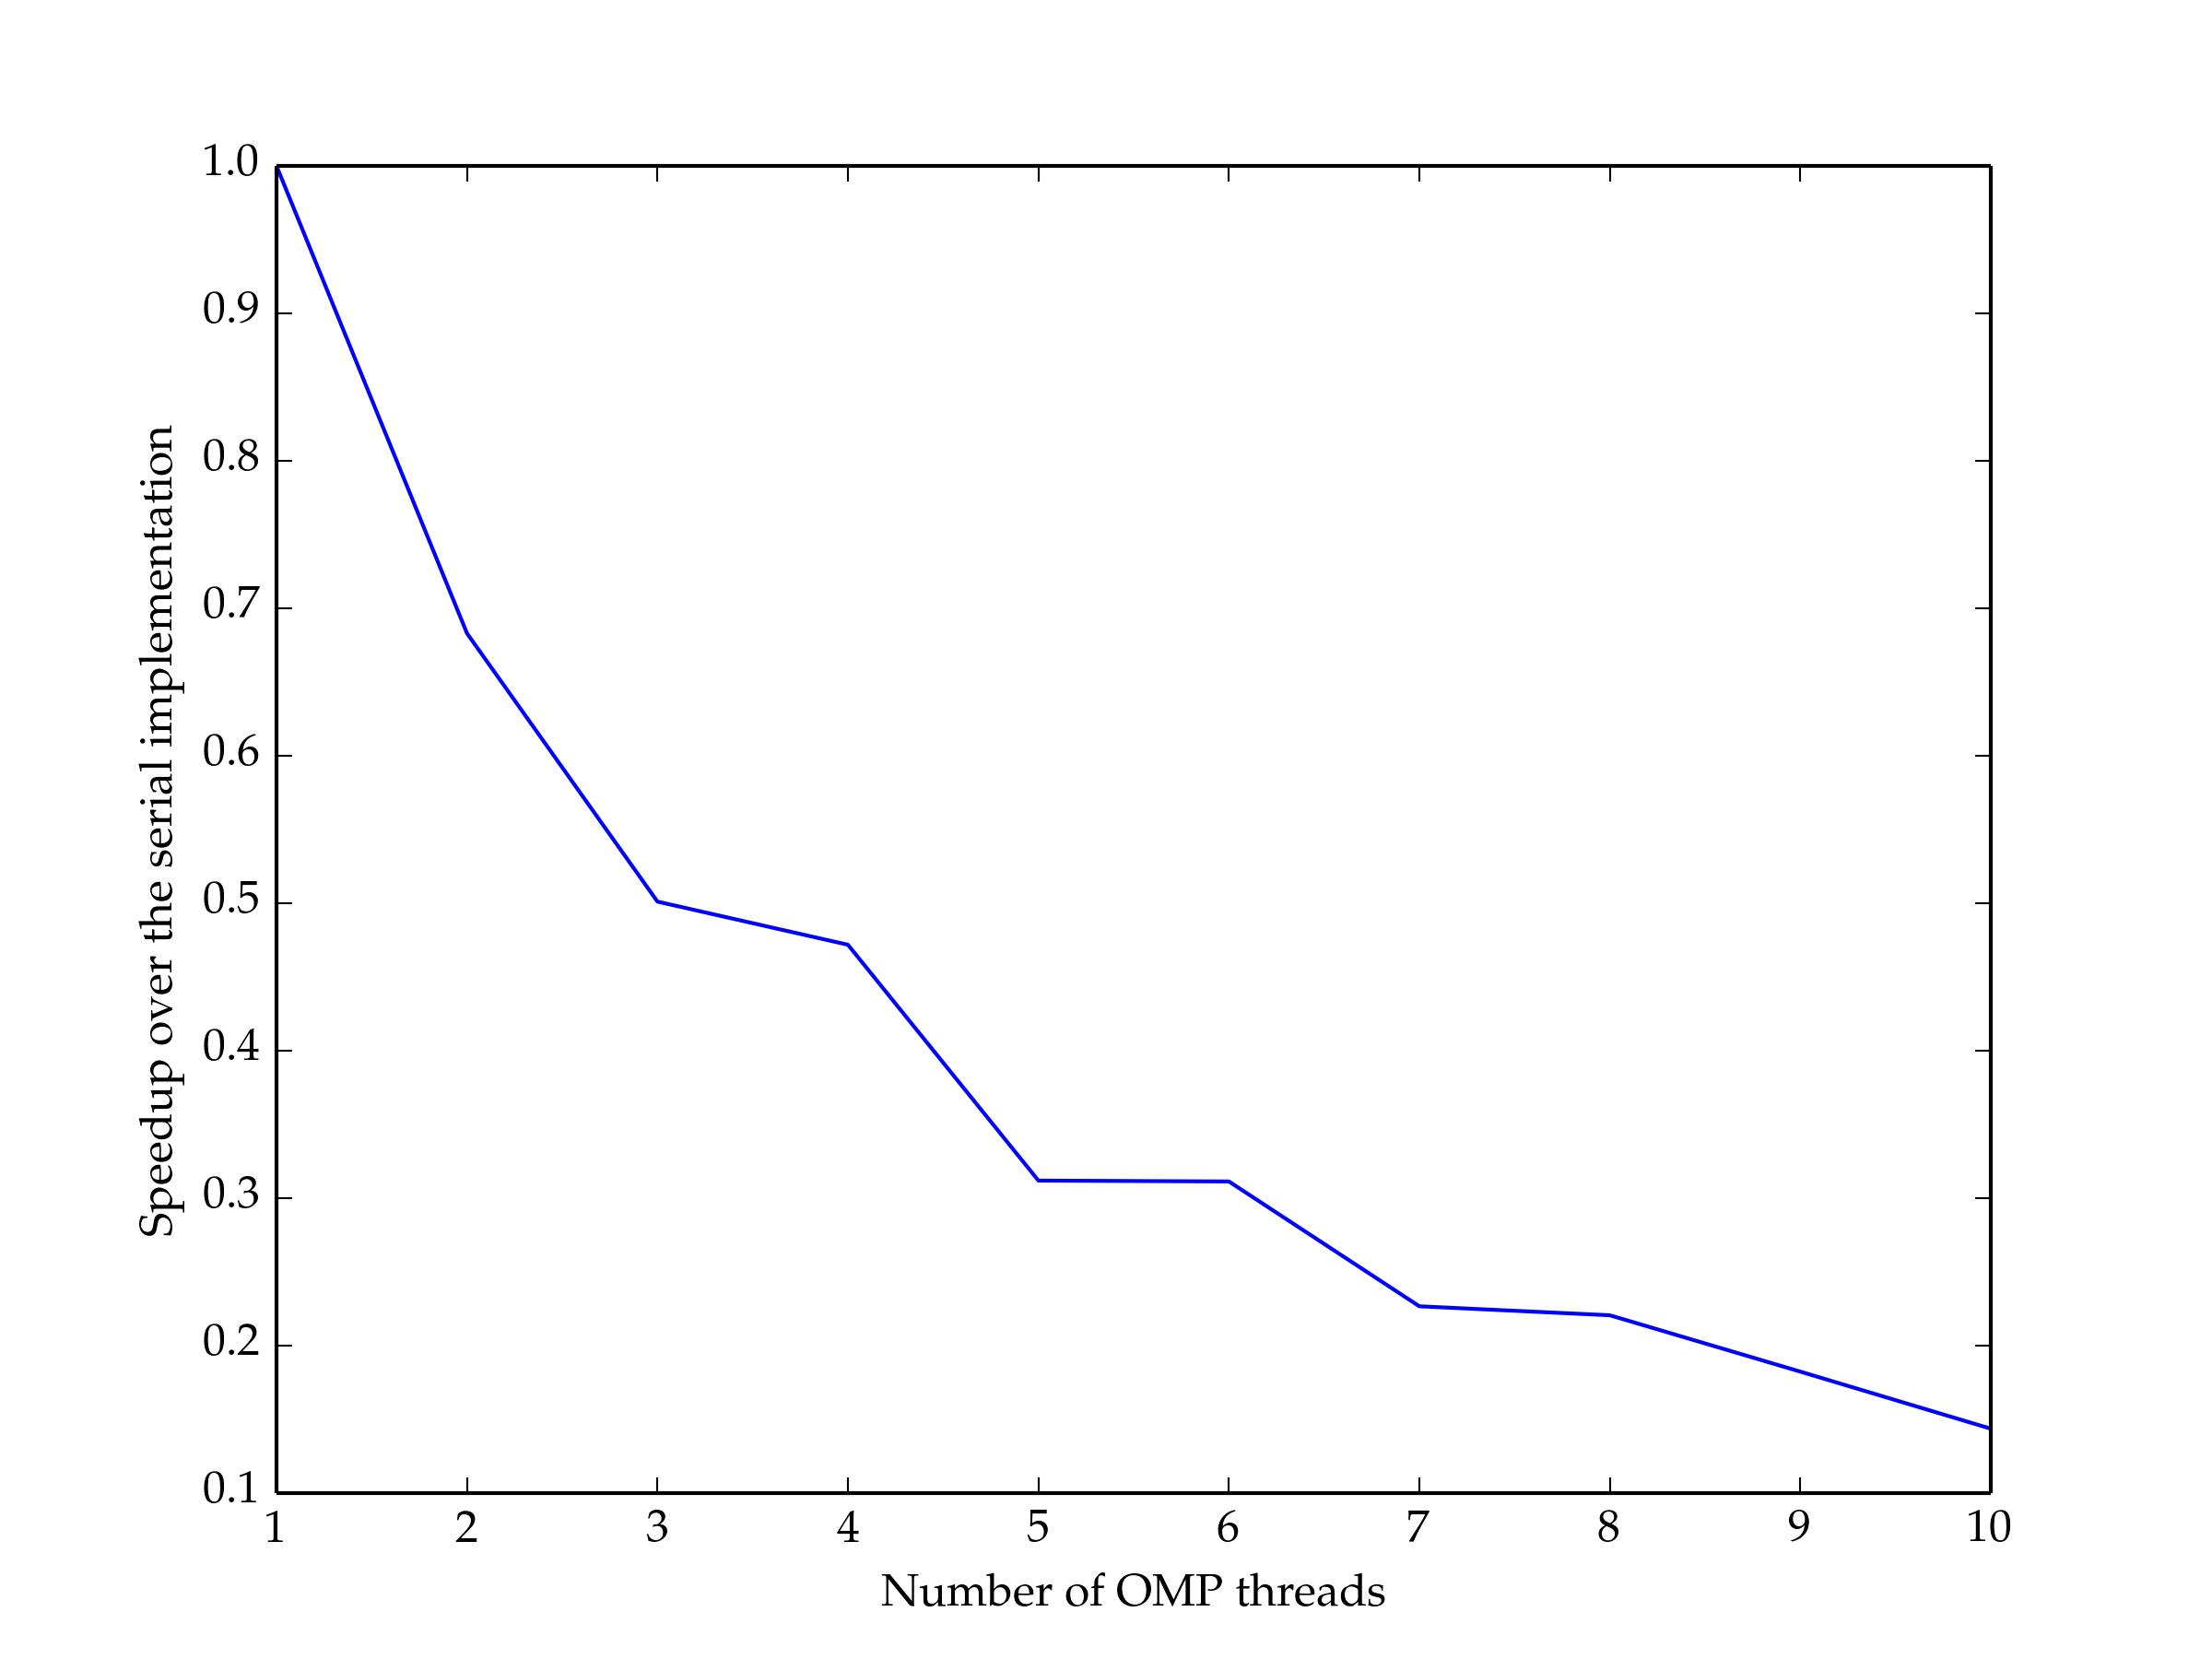
\includegraphics[width=0.9\textwidth]{./weak_scaling/weak_scaling.png}
    \caption{Speedup as a function of the number of threads}
    \label{fig:weak_scaling_dd}
\end{figure} 

\begin{thebibliography}{9}
\bibitem{vectorization} 
Data Alignment to Assist Vectorization. (n.d.). Retrieved September 30, 2015, from \url{https://software.intel.com/en-us/articles/data-alignment-to-assist-vectorization}

\bibitem{openmp}
Yliluoma, J. (n.d.). Guide into OpenMP: Easy multithreading programming for C. Retrieved October 19, 2015, from \url{http://bisqwit.iki.fi/story/howto/openmp/}

\end{thebibliography}

 
 
\end{document}
